% !TeX document-id = {8c6be429-7d79-4ce7-90ca-06d13b6696e5}
% !TeX TXS-program:bibliography = txs:///biber
\documentclass[14pt, russian]{scrartcl}
\let\counterwithout\relax
\let\counterwithin\relax
%\usepackage{lmodern}
\usepackage{float}
\usepackage{xcolor}
\usepackage{extsizes}
\usepackage{subfig}
\usepackage[export]{adjustbox}
\usepackage{tocvsec2} % возможность менять учитываемую глубину разделов в оглавлении
\usepackage[subfigure]{tocloft}
\usepackage[newfloat]{minted}
\setminted[text]{frame=single,fontsize = \footnotesize, linenos, xleftmargin = 1.5em, breaklines}
\setminted[rust]{frame=single,fontsize = \footnotesize, linenos, xleftmargin = 1.5em, breaklines}
\setminted[yaml]{frame=single,fontsize = \footnotesize, linenos, xleftmargin = 1.5em, breaklines}
\setminted[python]{frame=single,fontsize = \footnotesize, linenos, xleftmargin = 1.5em, breaklines}
\AtBeginEnvironment{figure}{\vspace{0.5cm}}
\AtBeginEnvironment{table}{\vspace{0.5cm}}
\AtBeginEnvironment{listing}{\vspace{0.5cm}}
\AtBeginEnvironment{minted}{\vspace{-0.5cm}}
\newenvironment{longlisting}{\captionsetup{type=listing}}{}
%\AfterEndEnvironment{minted}{\vspace{-1cm}}
\captionsetup[listing]{position=top}
\usepackage{array}
\usepackage{fancyvrb}
\usepackage{ulem,bm,mathrsfs,ifsym} %зачеркивания, особо жирный стиль и RSFS начертание
\usepackage{sectsty} % переопределение стилей подразделов
%%%%%%%%%%%%%%%%%%%%%%%

\newcolumntype{C}{>{\centering\arraybackslash}m{5em}}

%%% Поля и разметка страницы %%%
\usepackage{pdflscape}                              % Для включения альбомных страниц
\usepackage{geometry}                               % Для последующего задания полей
\geometry{a4paper,tmargin=2cm,bmargin=2cm,lmargin=3cm,rmargin=1cm} % тоже самое, но лучше
\newcommand*\lsin{\lstinline[columns=fixed]}

%%% Математические пакеты %%%
\usepackage{amsthm,amsfonts,amsmath,amssymb,amscd}  % Математические дополнения от AMS
\usepackage{mathtools}                              % Добавляет окружение multlined
\usepackage[perpage]{footmisc}
%\usepackage{times}

%%%% Установки для размера шрифта 14 pt %%%%
%% Формирование переменных и констант для сравнения (один раз для всех подключаемых файлов)%%
%% должно располагаться до вызова пакета fontspec или polyglossia, потому что они сбивают его работу
%\newlength{\curtextsize}
%\newlength{\bigtextsize}
%\setlength{\bigtextsize}{13pt}
\KOMAoptions{fontsize=14pt}

\makeatletter
\def\showfontsize{\f@size{} point}
\makeatother

%\makeatletter
%\show\f@size                                       % неплохо для отслеживания, но вызывает стопорение процесса, если документ компилируется без команды  -interaction=nonstopmode 
%\setlength{\curtextsize}{\f@size pt}
%\makeatother

%шрифт times
\usepackage{tempora}
%\usepackage{pscyr}
%\setmainfont[Ligatures={TeX,Historic}]{Times New Roman}

   %%% Решение проблемы копирования текста в буфер кракозябрами
%    \input glyphtounicode.tex
%    \input glyphtounicode-cmr.tex %from pdfx package
%    \pdfgentounicode=1
    \usepackage{cmap}                               % Улучшенный поиск русских слов в полученном pdf-файле
    \usepackage[T1]{fontenc}                       % Поддержка русских букв
    \usepackage[utf8]{inputenc}                     % Кодировка utf8
    \usepackage[english, main=russian]{babel}            % Языки: русский, английский
%   \IfFileExists{pscyr.sty}{\usepackage{pscyr}}{}  % Красивые русские шрифты
%\renewcommand{\rmdefault}{ftm}
%%% Оформление абзацев %%%
\usepackage{indentfirst}                            % Красная строка
%\usepackage{eskdpz}

%%% Таблицы %%%
\usepackage{longtable}                              % Длинные таблицы
\usepackage{multirow,makecell,array}                % Улучшенное форматирование таблиц
\usepackage{booktabs}                               % Возможность оформления таблиц в классическом книжном стиле (при правильном использовании не противоречит ГОСТ)

%%% Общее форматирование
\usepackage{soulutf8}                               % Поддержка переносоустойчивых подчёркиваний и зачёркиваний
\usepackage{icomma}                                 % Запятая в десятичных дробях



%%% Изображения %%%
\usepackage{graphicx}                               % Подключаем пакет работы с графикой
\graphicspath{{./images}}
\usepackage{wrapfig}

%%% Списки %%%
\usepackage{enumitem}

%%% Подписи %%%
\usepackage{caption}                                % Для управления подписями (рисунков и таблиц) % Может управлять номерами рисунков и таблиц с caption %Иногда может управлять заголовками в списках рисунков и таблиц
%% Использование:
%\begin{table}[h!]\ContinuedFloat - чтобы не переключать счетчик
%\captionsetup{labelformat=continued}% должен стоять до самого caption
%\caption{}
% либо ручками \caption*{Продолжение таблицы~\ref{...}.} :)

%%% Интервалы %%%
\addto\captionsrussian{%
  \renewcommand{\listingname}{Листинг}%
}
%%% Счётчики %%%
\usepackage[figure,table,section]{totalcount}               % Счётчик рисунков и таблиц
\DeclareTotalCounter{lstlisting}
\usepackage{totcount}                               % Пакет создания счётчиков на основе последнего номера подсчитываемого элемента (может требовать дважды компилировать документ)
\usepackage{totpages}                               % Счётчик страниц, совместимый с hyperref (ссылается на номер последней страницы). Желательно ставить последним пакетом в преамбуле

%%% Продвинутое управление групповыми ссылками (пока только формулами) %%%
%% Кодировки и шрифты %%%

%   \newfontfamily{\cyrillicfont}{Times New Roman}
%   \newfontfamily{\cyrillicfonttt}{CMU Typewriter Text}
	%\setmainfont{Times New Roman}
	%\newfontfamily\cyrillicfont{Times New Roman}
	%\setsansfont{Times New Roman}                    %% задаёт шрифт без засечек
%	\setmonofont{Liberation Mono}               %% задаёт моноширинный шрифт
%    \IfFileExists{pscyr.sty}{\renewcommand{\rmdefault}{ftm}}{}
%%% Интервалы %%%
%linespread-реализация ближе к реализации полуторного интервала в ворде.
%setspace реализация заточена под шрифты 10, 11, 12pt, под остальные кегли хуже, но всё же ближе к типографской классике. 
\linespread{1.3}                    % Полуторный интервал (ГОСТ Р 7.0.11-2011, 5.3.6)
%\renewcommand{\@biblabel}[1]{#1}

%%% Гиперссылки %%%
\usepackage{hyperref}

%%% Выравнивание и переносы %%%
\sloppy                             % Избавляемся от переполнений
\clubpenalty=10000                  % Запрещаем разрыв страницы после первой строки абзаца
\widowpenalty=10000                 % Запрещаем разрыв страницы после последней строки абзаца

\makeatletter % малые заглавные, small caps shape
\let\@@scshape=\scshape
\renewcommand{\scshape}{%
  \ifnum\strcmp{\f@series}{bx}=\z@
    \usefont{T1}{cmr}{bx}{sc}%
  \else
    \ifnum\strcmp{\f@shape}{it}=\z@
      \fontshape{scsl}\selectfont
    \else
      \@@scshape
    \fi
  \fi}
\makeatother

%%% Подписи %%%
%\captionsetup{%
%singlelinecheck=off,                % Многострочные подписи, например у таблиц
%skip=2pt,                           % Вертикальная отбивка между подписью и содержимым рисунка или таблицы определяется ключом
%justification=centering,            % Центрирование подписей, заданных командой \caption
%}
%%%        Подключение пакетов                 %%%
\usepackage{ifthen}                 % добавляет ifthenelse
%%% Инициализирование переменных, не трогать!  %%%
\newcounter{intvl}
\newcounter{otstup}
\newcounter{contnumeq}
\newcounter{contnumfig}
\newcounter{contnumtab}
\newcounter{pgnum}
\newcounter{bibliosel}
\newcounter{chapstyle}
\newcounter{headingdelim}
\newcounter{headingalign}
\newcounter{headingsize}
\newcounter{tabcap}
\newcounter{tablaba}
\newcounter{tabtita}
%%%%%%%%%%%%%%%%%%%%%%%%%%%%%%%%%%%%%%%%%%%%%%%%%%

%%% Область упрощённого управления оформлением %%%

%% Интервал между заголовками и между заголовком и текстом
% Заголовки отделяют от текста сверху и снизу тремя интервалами (ГОСТ Р 7.0.11-2011, 5.3.5)
\setcounter{intvl}{3}               % Коэффициент кратности к размеру шрифта

%% Отступы у заголовков в тексте
\setcounter{otstup}{0}              % 0 --- без отступа; 1 --- абзацный отступ

%% Нумерация формул, таблиц и рисунков
\setcounter{contnumeq}{1}           % Нумерация формул: 0 --- пораздельно (во введении подряд, без номера раздела); 1 --- сквозная нумерация по всей диссертации
\setcounter{contnumfig}{1}          % Нумерация рисунков: 0 --- пораздельно (во введении подряд, без номера раздела); 1 --- сквозная нумерация по всей диссертации
\setcounter{contnumtab}{1}          % Нумерация таблиц: 0 --- пораздельно (во введении подряд, без номера раздела); 1 --- сквозная нумерация по всей диссертации

%% Оглавление
\setcounter{pgnum}{0}               % 0 --- номера страниц никак не обозначены; 1 --- Стр. над номерами страниц (дважды компилировать после изменения)

%% Библиография
\setcounter{bibliosel}{1}           % 0 --- встроенная реализация с загрузкой файла через движок bibtex8; 1 --- реализация пакетом biblatex через движок biber

%% Текст и форматирование заголовков
\setcounter{chapstyle}{1}           % 0 --- разделы только под номером; 1 --- разделы с названием "Глава" перед номером
\setcounter{headingdelim}{1}        % 0 --- номер отделен пропуском в 1em или \quad; 1 --- номера разделов и приложений отделены точкой с пробелом, подразделы пропуском без точки; 2 --- номера разделов, подразделов и приложений отделены точкой с пробелом.

%% Выравнивание заголовков в тексте
\setcounter{headingalign}{0}        % 0 --- по центру; 1 --- по левому краю

%% Размеры заголовков в тексте
\setcounter{headingsize}{0}         % 0 --- по ГОСТ, все всегда 14 пт; 1 --- пропорционально изменяющийся размер в зависимости от базового шрифта

%% Подпись таблиц
\setcounter{tabcap}{0}              % 0 --- по ГОСТ, номер таблицы и название разделены тире, выровнены по левому краю, при необходимости на нескольких строках; 1 --- подпись таблицы не по ГОСТ, на двух и более строках, дальнейшие настройки: 
%Выравнивание первой строки, с подписью и номером
\setcounter{tablaba}{2}             % 0 --- по левому краю; 1 --- по центру; 2 --- по правому краю
%Выравнивание строк с самим названием таблицы
\setcounter{tabtita}{1}             % 0 --- по левому краю; 1 --- по центру; 2 --- по правому краю

%%% Рисунки %%%
\DeclareCaptionLabelSeparator*{emdash}{~--- }             % (ГОСТ 2.105, 4.3.1)
\captionsetup[figure]{labelsep=emdash,font=onehalfspacing,position=bottom}

%%% Таблицы %%%
\ifthenelse{\equal{\thetabcap}{0}}{%
    \newcommand{\tabcapalign}{\raggedright}  % по левому краю страницы или аналога parbox
}

\ifthenelse{\equal{\thetablaba}{0} \AND \equal{\thetabcap}{1}}{%
    \newcommand{\tabcapalign}{\raggedright}  % по левому краю страницы или аналога parbox
}

\ifthenelse{\equal{\thetablaba}{1} \AND \equal{\thetabcap}{1}}{%
    \newcommand{\tabcapalign}{\centering}    % по центру страницы или аналога parbox
}

\ifthenelse{\equal{\thetablaba}{2} \AND \equal{\thetabcap}{1}}{%
    \newcommand{\tabcapalign}{\raggedleft}   % по правому краю страницы или аналога parbox
}

\ifthenelse{\equal{\thetabtita}{0} \AND \equal{\thetabcap}{1}}{%
    \newcommand{\tabtitalign}{\raggedright}  % по левому краю страницы или аналога parbox
}

\ifthenelse{\equal{\thetabtita}{1} \AND \equal{\thetabcap}{1}}{%
    \newcommand{\tabtitalign}{\centering}    % по центру страницы или аналога parbox
}

\ifthenelse{\equal{\thetabtita}{2} \AND \equal{\thetabcap}{1}}{%
    \newcommand{\tabtitalign}{\raggedleft}   % по правому краю страницы или аналога parbox
}

\DeclareCaptionFormat{tablenocaption}{\tabcapalign #1\strut}        % Наименование таблицы отсутствует
\ifthenelse{\equal{\thetabcap}{0}}{%
    \DeclareCaptionFormat{tablecaption}{\tabcapalign #1#2#3}
    \captionsetup[table]{labelsep=emdash}                       % тире как разделитель идентификатора с номером от наименования
}{%
    \DeclareCaptionFormat{tablecaption}{\tabcapalign #1#2\par%  % Идентификатор таблицы на отдельной строке
        \tabtitalign{#3}}                                       % Наименование таблицы строкой ниже
    \captionsetup[table]{labelsep=space}                        % пробельный разделитель идентификатора с номером от наименования
}
\captionsetup[table]{format=tablecaption,singlelinecheck=off,font=onehalfspacing,position=top,skip=-5pt}  % многострочные наименования и прочее
\DeclareCaptionLabelFormat{continued}{Продолжение таблицы~#2}
\setlength{\belowcaptionskip}{.2cm}
\setlength{\intextsep}{0ex}

%%% Подписи подрисунков %%%
\renewcommand{\thesubfigure}{\asbuk{subfigure}}           % Буквенные номера подрисунков
\captionsetup[subfigure]{font={normalsize},               % Шрифт подписи названий подрисунков (не отличается от основного)
    labelformat=brace,                                    % Формат обозначения подрисунка
    justification=centering,                              % Выключка подписей (форматирование), один из вариантов            
}
%\DeclareCaptionFont{font12pt}{\fontsize{12pt}{13pt}\selectfont} % объявляем шрифт 12pt для использования в подписях, тут же надо интерлиньяж объявлять, если не наследуется
%\captionsetup[subfigure]{font={font12pt}}                 % Шрифт подписи названий подрисунков (всегда 12pt)

%%% Настройки гиперссылок %%%

\definecolor{linkcolor}{rgb}{0.0,0,0}
\definecolor{citecolor}{rgb}{0,0.0,0}
\definecolor{urlcolor}{rgb}{0,0,0}

\hypersetup{
    linktocpage=true,           % ссылки с номера страницы в оглавлении, списке таблиц и списке рисунков
%    linktoc=all,                % both the section and page part are links
%    pdfpagelabels=false,        % set PDF page labels (true|false)
    plainpages=true,           % Forces page anchors to be named by the Arabic form  of the page number, rather than the formatted form
    colorlinks,                 % ссылки отображаются раскрашенным текстом, а не раскрашенным прямоугольником, вокруг текста
    linkcolor={linkcolor},      % цвет ссылок типа ref, eqref и подобных
    citecolor={citecolor},      % цвет ссылок-цитат
    urlcolor={urlcolor},        % цвет гиперссылок
    pdflang={ru},
}
\urlstyle{same}
%%% Шаблон %%%
%\DeclareRobustCommand{\todo}{\textcolor{red}}       % решаем проблему превращения названия цвета в результате \MakeUppercase, http://tex.stackexchange.com/a/187930/79756 , \DeclareRobustCommand protects \todo from expanding inside \MakeUppercase
\setlength{\parindent}{2.5em}                       % Абзацный отступ. Должен быть одинаковым по всему тексту и равен пяти знакам (ГОСТ Р 7.0.11-2011, 5.3.7).

%%% Списки %%%
% Используем дефис для ненумерованных списков (ГОСТ 2.105-95, 4.1.7)
%\renewcommand{\labelitemi}{\normalfont\bfseries~{---}} 
\renewcommand{\labelitemi}{\bfseries~{---}} 
\setlist{nosep,%                                    % Единый стиль для всех списков (пакет enumitem), без дополнительных интервалов.
    labelindent=\parindent,leftmargin=*%            % Каждый пункт, подпункт и перечисление записывают с абзацного отступа (ГОСТ 2.105-95, 4.1.8)
}
%%%%%%%%%%%%%%%%%%%%%%
%\usepackage{xltxtra} % load xunicode

\usepackage{ragged2e}
\usepackage[explicit]{titlesec}
\usepackage{placeins}
\usepackage{xparse}
\usepackage{csquotes}

\usepackage{listingsutf8}
\usepackage{url} %пакеты расширений
\usepackage{algorithm}
\usepackage[noend]{algpseudocode}
\usepackage{blkarray}
\usepackage{chngcntr}
\usepackage{tabularx}
\usepackage[backend=biber, 
    maxnames=5,
    bibstyle=gost-numeric,
    citestyle=nature]{biblatex}
\newcommand*\template[1]{\text{<}#1\text{>}}
\addbibresource{biblio.bib}
\renewcommand{\mkgostheading}[1]{#1}
\renewcommand*{\newblockpunct}{\addperiod\addnbspace\textendash\space\bibsentence}
\renewcommand*{\bibrangedash}{\text{\textendash}}
\titleformat{name=\section,numberless}[block]{\normalfont\Large\centering}{}{0em}{#1}
\titleformat{\section}[block]{\normalfont\Large\bfseries\raggedright}{}{0em}{\thesection\hspace{0.25em}#1}
\titleformat{\subsection}[block]{\normalfont\Large\bfseries\raggedright}{}{0em}{\thesubsection\hspace{0.25em}#1}
\titleformat{\subsubsection}[block]{\normalfont\large\bfseries\raggedright}{}{0em}{\thesubsubsection\hspace{0.25em}#1}

\let\Algorithm\algorithm
\renewcommand\algorithm[1][]{\Algorithm[#1]\setstretch{1.5}}
%\renewcommand{\listingscaption}{Листинг}

\usepackage{pifont}
\usepackage{calc}
\usepackage{suffix}
\usepackage[none]{hyphenat}
\usepackage{csquotes}
\DeclareQuoteStyle{russian}
    {\guillemotleft}{\guillemotright}[0.025em]
    {\quotedblbase}{\textquotedblleft}
\ExecuteQuoteOptions{style=russian}
\newcommand{\enq}[1]{\enquote{#1}}  
\newcommand{\eng}[1]{\begin{english}#1\end{english}}
% Подчиненные счетчики в окружениях http://old.kpfu.ru/journals/izv_vuz/arch/sample1251.tex
\newcounter{cTheorem} 
\newcounter{cDefinition}
\newcounter{cConsequent}
\newcounter{cExample}
\newcounter{cLemma}
\newcounter{cConjecture}
\newtheorem{Theorem}{Теорема}[cTheorem]
\newtheorem{Definition}{Определение}[cDefinition]
\newtheorem{Consequent}{Следствие}[cConsequent]
\newtheorem{Example}{Пример}[cExample]
\newtheorem{Lemma}{Лемма}[cLemma]
\newtheorem{Conjecture}{Гипотеза}[cConjecture]

\renewcommand{\theTheorem}{\arabic{Theorem}}
\renewcommand{\theDefinition}{\arabic{Definition}}
\renewcommand{\theConsequent}{\arabic{Consequent}}
\renewcommand{\theExample}{\arabic{Example}}
\renewcommand{\theLemma}{\arabic{Lemma}}
\renewcommand{\theConjecture}{\arabic{Conjecture}}
%\makeatletter
\NewDocumentCommand{\Newline}{}{\text{\\}}
\newcommand{\sequence}[2]{\ensuremath \left(#1,\ \dots,\ #2\right)}

\definecolor{mygreen}{rgb}{0,0.6,0}
\definecolor{mygray}{rgb}{0.5,0.5,0.5}
\definecolor{mymauve}{rgb}{0.58,0,0.82}
\renewcommand{\listalgorithmname}{Список алгоритмов}
\floatname{algorithm}{Листинг}



\renewcommand{\lstlistingname}{Листинг}
\DeclareCaptionFormat{listing}{#1 --- #3}
\captionsetup[listing]{format=listing, singlelinecheck=false, labelsep=colon}




\renewcommand{\thealgorithm}{\arabic{algorithm}}

\newcommand{\refAlgo}[1]{(листинг \ref{#1})}
\newcommand{\refImage}[1]{(рисунок \ref{#1})}

\renewcommand{\theenumi}{\arabic{enumi}.}% Меняем везде перечисления на цифра.цифра	
\renewcommand{\labelenumi}{\arabic{enumi}.}% Меняем везде перечисления на цифра.цифра
\renewcommand{\theenumii}{\arabic{enumii}}% Меняем везде перечисления на цифра.цифра
\renewcommand{\labelenumii}{(\arabic{enumii})}% Меняем везде перечисления на цифра.цифра
\renewcommand{\theenumiii}{\roman{enumiii}}% Меняем везде перечисления на цифра.цифра
\renewcommand{\labelenumiii}{(\roman{enumiii})}% Меняем везде перечисления на цифра.цифра
%\newfontfamily\AnkaCoder[Path=src/fonts/]{AnkaCoder-r.ttf}
\renewcommand{\labelitemi}{---}
\renewcommand{\labelitemii}{---}

\def\customfigurename{Рисунок}
% Define a new counter for the custom figures
\newcounter{customfigurecounter}
\renewcommand{\thecustomfigurecounter}{A.\arabic{customfigurecounter}}

% Define a new float environment for the custom figures
\DeclareFloatingEnvironment[fileext=cust]{customfigure}

% Redefine the caption format for the custom figures
\DeclareCaptionLabelFormat{customlabel}{#1~\thecustomfigurecounter}
\captionsetup[customfigure]{labelformat=customlabel, labelsep=emdash,font=onehalfspacing,position=bottom}


\newcounter{alisting}
\lstnewenvironment{alisting}[2]{
    \renewcommand\lstlistingname{Листинг}
    \setcounter{lstlisting}{А.\value{alisting}}
    \lstset{ ... }
} {\addtocounter{alisting}{1}}

%\usepackage{courier}



\makeatletter
\def\p@subsection{}
\def\p@subsubsection{\thesection\,\thesubsection\,}
\makeatother
\newcommand{\prog}[1]{{\ttfamily\small#1}}
\newcommand{\anonsection}[1]{\cleardoublepage
\phantomsection
\addcontentsline{toc}{section}{\protect\numberline{}#1}
\section*{#1}\vspace*{2.5ex} % По госту положены 3 пустые строки после заголовка ненумеруемого раздела
}
\newcommand{\sectionbreak}{\clearpage}
\renewcommand{\sectionfont}{\normalsize} % Сбиваем стиль оглавления в стандартный
\renewcommand{\cftsecleader}{\cftdotfill{\cftdotsep}} % Точки в оглавлении напротив разделов

\renewcommand{\cftsecfont}{\normalfont\large} % Переключение на times в содержании
\renewcommand{\cftsubsecfont}{\normalfont\large} % Переключение на times в содержании

\usepackage{caption} 
%\captionsetup[table]{justification=raggedleft} 
%\captionsetup[figure]{justification=centering,labelsep=endash}2111111
\usepackage{amsmath}    % \bar    (матрицы и проч. ...)
\usepackage{amsfonts}   % \mathbb (символ для множества действительных чисел и проч. ...)
\usepackage{mathtools}  % \abs, \norm
    \DeclarePairedDelimiter\abs{\lvert}{\rvert} % операция модуля
    \DeclarePairedDelimiter\norm{\lVert}{\rVert} % операция нормы
\DeclareTextCommandDefault{\textvisiblespace}{%
  \mbox{\kern.06em\vrule \@height.3ex}%
  \vbox{\hrule \@width.3em}%
  \hbox{\vrule \@height.3ex}}    
\newsavebox{\spacebox}
\begin{lrbox}{\spacebox}
\verb*! !
\end{lrbox}
\newcommand{\aspace}{\usebox{\spacebox}}
\DeclareTotalCounter{listing}
    
\begin{document}
\sloppy

\def\figurename{Рисунок}


\begin{titlepage}
\thispagestyle{empty}
\newpage

\vspace*{-30pt}
\hspace{-45pt}
\begin{minipage}{0.17\textwidth}
\hspace*{-20pt}\centering
\includegraphics[width=1.3\textwidth]{images/Emblem.png}
\end{minipage}
\begin{minipage}{0.82\textwidth}\small \textbf{
\vspace*{-0.7ex}
\hspace*{-10pt}\centerline{Министерство науки и высшего образования Российской Федерации}
\vspace*{-0.7ex}
\centerline{Федеральное государственное бюджетное образовательное учреждение }
\vspace*{-0.7ex}
\centerline{высшего образования}
\vspace*{-0.7ex}
\centerline{<<Московский государственный технический университет}
\vspace*{-0.7ex}
\centerline{имени Н.Э. Баумана}
\vspace*{-0.7ex}
\centerline{(национальный исследовательский университет)>>}
\vspace*{-0.7ex}
\centerline{(МГТУ им. Н.Э. Баумана)}}
\end{minipage}

\vspace{-2pt}
\hspace{-34.5pt}\rule{\textwidth}{2.5pt}

\vspace*{-20.3pt}
\hspace{-34.5pt}\rule{\textwidth}{0.4pt}
\vspace{0.5ex}
\noindent \small ФАКУЛЬТЕТ\hspace{80pt} <<Информатика и системы управления>>

\vspace*{-16pt}
\hspace{35pt}\rule{0.855\textwidth}{0.4pt}

\vspace{0.5ex}
\noindent \small КАФЕДРА\hspace{50pt} <<Теоретическая информатика и компьютерные технологии>>

\vspace*{-16pt}
\hspace{25pt}\rule{0.875\textwidth}{0.4pt}
 
 
\vspace{3em}
 
\begin{center}
\Large \bf{ОТЁТ ПО ПРЕДДИПЛОМНОЙ \\ ПРАКТИКЕ\\}
\end{center}

% \vspace*{-6ex} 
% \begin{center}
% \Large{\textit{\textbf{}}}

% \vspace*{-3ex}
% \rule{0.9\textwidth}{1.2pt}

% \Large{\textit{\textbf{}}}

% \vspace*{-3ex}
% \rule{0.9\textwidth}{1.2pt}

% \vspace*{-0.2ex}
% \rule{0.9\textwidth}{1.2pt}

% \vspace*{-0.2ex}
% \rule{0.9\textwidth}{1.2pt}

% \vspace*{-0.2ex}
% \rule{0.9\textwidth}{1.2pt}
% \end{center}

% \vspace{\fill}
 

% \newlength{\ML}
% \settowidth{\ML}{«\underline{\hspace{0.7cm}}» \underline{\hspace{2cm}}}

\noindent Студент \underline{\hspace{15.3cm}}

\vspace{-2.1ex}
\noindent\hspace{7.0cm}\scriptsize{(Фамилия, Имя, Отчество)}\normalsize
\bigskip

\noindent Группа \underline{\hspace{2.0cm}} \hfill 

\vspace{-2.1ex}
\noindent\hspace{7.0cm}
\bigskip

\noindent Тип практики \underline{\hspace{14.0cm}} \hfill 

\vspace{-2.1ex}
\noindent\hspace{7.0cm}
\bigskip

\noindent Название предприятия \underline{\hspace{1.5cm} МГТУ им. Н.Э. Баумана\hspace{1.5cm}} \hfill 

\vspace{-2.1ex}
\noindent\hspace{7.0cm}
\bigskip

\vspace{1.5cm}

\noindent Студент \underline{\hspace{1.5cm}} \hfill \underline{\hspace{4cm}}\quad
\underline{\hspace{4cm}}

\vspace{-2.1ex}
\noindent\hspace{9ex}\scriptsize{(Группа)}\normalsize\hspace{160pt}\hspace{2ex}\scriptsize{(Подпись, дата)}\normalsize\hspace{30pt}\hspace{6ex}\scriptsize{(И.О. Фамилия)}\normalsize
\bigskip

\noindent Рекомендуемая оценка \hfill \underline{\hspace{7.0cm}}

\vspace{-2ex}
\noindent\hspace{13.5ex}
\bigskip

\noindent Руководитель практики \hfill \underline{\hspace{4cm}}\quad
\underline{\hspace{4cm}}

\vspace{-2ex}
\noindent\hspace{13.5ex}\normalsize\hspace{170pt}\hspace{2ex}\scriptsize{(Подпись, дата)}\normalsize\hspace{30pt}\hspace{6ex}\scriptsize{(И.О. Фамилия)}\normalsize
\bigskip

\noindent Оценка \hfill \underline{\hspace{7.0cm}}

\vspace{-2ex}
\noindent\hspace{13.5ex}
\bigskip
\vfill

% \noindent Студент \hfill \underline{\hspace{4.76cm}Головкин Дмитрий Сергеевич\hspace{4.76cm}}

% \vspace{-2.1ex}
% \noindent\hspace{8.0cm}\scriptsize{(Фамилия, Имя, Отчество)}\normalsize
% \bigskip

% \noindent Группа \underline{\hspace{0.3cm}ИУ9-82Б\hspace{0.3cm}} \hfill 

% \vspace{-2.1ex}
% \noindent\hspace{7.0cm}
% \bigskip

% \noindent Тип практики \hfill \underline{\hspace{5.4cm}Преддипломная\hspace{5.4cm}} \hfill 

% \vspace{-2.1ex}
% \noindent\hspace{7.0cm}
% \bigskip

% \noindent Название предприятия \underline{\hspace{1.5cm}МГТУ им. Н.Э. Баумана\hspace{1.5cm}} \hfill 

% \vspace{-2.1ex}
% \noindent\hspace{7.0cm}
% \bigskip

% \vspace{1.5cm}

% \noindent Студент \underline{\hspace{0.2cm} ИУ9-82Б\hspace{0.2cm}} \hfill \underline{\hspace{4cm}}\quad
% \underline{\hspace{0.5cm}Д.С. Головкин\hspace{0.5cm}}

% \vspace{-2.1ex}
% \noindent\hspace{10ex}\scriptsize{(Группа)}\normalsize\hspace{160pt}\hspace{2ex}\scriptsize{(Подпись, дата)}\normalsize\hspace{30pt}\hspace{6ex}\scriptsize{(И.О. Фамилия)}\normalsize
% \bigskip

% \noindent Рекомендуемая оценка \hfill \underline{\hspace{7.0cm}}

% \vspace{-2ex}
% \noindent\hspace{13.5ex}
% \bigskip

% \noindent Руководитель практики \hfill \underline{\hspace{4cm}}\quad
% \underline{\hspace{0.35cm}А.В. Коновалов\hspace{0.35cm}}

% \vspace{-2ex}
% \noindent\hspace{13.5ex}\normalsize\hspace{170pt}\hspace{2ex}\scriptsize{(Подпись, дата)}\normalsize\hspace{30pt}\hspace{6ex}\scriptsize{(И.О. Фамилия)}\normalsize
% \bigskip

% \noindent Оценка \hfill \underline{\hspace{7.0cm}}

% \vspace{-2ex}
% \noindent\hspace{13.5ex}
% \bigskip
% \vfill

%\vspace{\fill}
 


\begin{center}
\textsl{2024 г.}
\end{center}
\end{titlepage}

%\renewcommand{\ttdefault}{pcr}

\setlength{\tabcolsep}{3pt}
\newpage
\setcounter{page}{2}
%----------------------------------------------------------------------------

%                  ОТСЮДА --- СОБСТВЕННО ТЕКСТ

%----------------------------------------------------------------------------
\section*{АННОТАЦИЯ}

Темой данной работы является <<Разработка программы анализа гиперспектральных изображений с помощью осцилляторных нейронных сетей>>. 
Работа состоит из~\pageref{TotPages} страниц и содержит \totalsections{} разделов, \totallistings{} листингов.

\newpage
\renewcommand\contentsname{\hfill{\normalfont{СОДЕРЖАНИЕ}}\hfill}  %Оглавление
\tableofcontents
\newpage
\anonsection{ВВЕДЕНИЕ}  %Введение

Цель данной работы -- разработка программы для сегментации целевых объектов на гиперспектральном изображении с помощью осцилляторных нейронных сетей. 
Необходимо разработать стратегию выбора спектральных каналов для улучшения работы программы. Также необходимо реализовать возможность использования различных модулей
и их комбинаций для обработки изображений. В конечном итоге необхождимо протестировать разработанную программу.
\newpage

\section{Постановка задачи}\label{sect:task_set}

Программа должна получать на вход набор флагов, по которым будет определяться дальнейшее поведение программы. Базовый вариант использование будет подразумевать
использование предзагруженного датасета гиперспектральных изобравжений и работы с ним. Цель программы состоит в сегментации обхекта определенного класса на 
гиперспектральном изображдении. Из предоставленного изображения случайным образом выбирается его часть,\
которая в дальнейшем будет обработана. Программа должна вывести маску сегментированного изображения, изначальное изображение, их пересечение и результат по 
одной из метрик, которые можно будет выбрать с помощью флагов. 

\section{Характеристика предприятия}

Производственная практика проходила с 13 мая по 27 мая 2024 года в МГТУ
им. Н.Э. Баумана.
МГТУ им. Н.Э. Баумана является одним из ведущих технических вузов
страны. Университет ведёт подготовку инженеров с 1830 года. На сегодняшний
день в университете обучают по большому количеству направлений. Выпускники
МГТУ становятся очень востребованными у работодателей на рынке труда. Ключевой особенностью обучения является сочетание теоретических и практических
знаний. Университет занимается научными исследованиями и разработками. Университет стал одним из единственных в России, которому агентство «Эксперт РА»
присвоило рейтинговый класс «В», означающий «очень высокий» уровень подготовки выпускников. Ежегодно университет входит в топ-300 мирового рейтинга
QS, и входит в пятерку лучших среди российских университетов.
Кафедра осуществляет подготовку дипломированных специалистов с квалификацией «Математик, системный программист» по программе высшего профессионального образования по специальности «Прикладная математика и информатика» со специализацией «Системное программирование».
Подготовка специалистов осуществляется по математическому и программному обеспечению высокотехнологичных областей техники и современных информационных технологий с уклоном в высокоэффективное программирование,
предусматривающее углублённые знания алгоритмов и приёмов решения задач по
прикладной математике и программированию.

\section{Реализация программы}

В данном разделе приведена реализация программы, выполняющей анализ гиперспектральных изображений с помощью осцилляторной нейронной сети.

В качестве языка программирования был выбран язык программирования Python. Данный выбор обусловлен существованием большого множества подключаемых библиотек,
поддержкой ООП, а также чрезвычайной простотой особенностей языка.

\subsection{Структура программы}

Программа разрабатывалась в репозитории с поддержкой системы контроля версий git.

Исходный код программы расположен в папке по пути \texttt{source/}. Функция main точки входа в программу расположена в файле \texttt{main.py}. В файле \texttt{dataset\_loader.py} 
и \texttt{datasets.py} расположены, соответсвенно, загрузчик различных датасетов и класс самого датасета, реализующий различные функции взаимодействия с данными.
В файлах \texttt{onn\_model.py}, \texttt{GaborGradScale.py} и \texttt{stimul.py} расположены классы, отвечающие за логику работы различных частей модели осцилляторной нейронной сети.
В файле \texttt{oscillators.py} описаны классы, реализующие логику работы составных элементов сети. В файле \texttt{pipelines.py} содержится класс для удобного управления процессом инициализации и работы нейронной сети.
В файле \texttt{hyperparams\_opt.py} содержатся функции и классы для проведения подбора гиперпараметров модели. В файле \texttt{utils.py} расположены вспомогательные функции и классы.

В папке по пути \texttt{tests/} расположены юнит-тесты программы.

В папке по пути \texttt{hyperparams/} расположены json файлы конфигурации параметров модели. 

\subsection{Параметры запуска программы}

Для поддержки параметров запуска программы и их парсинга использовалась библиотека argparse~\cite{1}. Выбор этой библиотеки объяняется ее простотой и предоставляемым функционалом.

Программа поддерживает следующие параметры запуска:

\begin{itemize}
    \item \texttt{dataset\_name} (строковый тип) -- устанавливает используемый датасет. При отсутсвии выбранного датасета в директории программы производится его загрузка;
    \item \texttt{hyperparams\_path} (строковый тип) -- путь до файла с гиперпараметрами;
    \item \texttt{optimize\_before\_run} (булевый тип) -- запуск программы с оптимизацией гиперпараметров;
    \item \texttt{metric} (строковый тип) -- метрика, по которой будет оценено качество сегментации;
    \item \texttt{segm\_filedir} (строковый тип) -- путь до директории с выходным файлом с результатами сегментации, без имя файла и расширения.
\end{itemize}

\subsection{Конвейер программы}

Общий конвейер программы находится в файле \texttt{pipelines.py} и описывается классом \texttt{OnnHyperPipeline} (см. Листинг 1). В этом классе расположены все методы для работы с данными и 
с моделями. Четыре основных метода это \texttt{add\_dataset} (см. Листинг 1), \texttt{create\_samples} (см. Листинг 1), \texttt{run} (см. Листинг 2) и \texttt{eval} (см. Листинг 3).

Метод \texttt{add\_dataset} выполняет вызов метода, отвечающего за загрузку датасета в классе \texttt{dataset\_loader}. Метод \texttt{create\_samples} выполняет разбиение полученного 
гиперспектрального изображения из датасета посредством вызова метода класса \texttt{HyperSpectralData} и далее вспомогательной функции \texttt{build\_dataset}. 
Метод \texttt{run} выполняет полную подготовку к запуску модели (вызов методов \texttt{add\_dataset} и \texttt{create\_samples}), а также осуществляет загрузку гиперпараметров из указанного 
в аргументах запуска файла и выполняет вызов функции \texttt{hyperparams\_opt} для оптимизации гиперпараметров.
Метод \texttt{eval} отвечает за обработку и сохранение результатов сегментации модели. Он вызывает вспомогательную функцию \texttt{evaluate\_best\_segmentation}.

\begin{listing}[H]
    \caption{Класс конвейера и некоторые методы}
    \label{lst:pipeline}
    \begin{minted}[frame=single, breaklines=True, fontsize = \footnotesize, linenos]{python}
class OnnHyperPipeline(HyperPipeline):
"""Pipeline class for implementing ONN workflow"""

    def __init__(self):
        super().__init__()
        self.dataset: HyperSpectralData
        self.model: OnnModel
        self.result: list[Result]
        self.params: Params

    def add_dataset(self, dataset_name='PaviaU', 
                          load_folder="./datasets"):
        data, gt, labels, ignored_labels, \
        rgb_bands, palette, num_of_bands = get_dataset(dataset_name,
                                                       load_folder)
        params = {'labels': labels, 
                'ignored_labels': ignored_labels,
                'rbg_bands': rgb_bands,
                'palette': palette,
                'num_of_bands': num_of_bands}
        self.dataset = HyperSpectralData(data, gt, **params)

    def get_data_info(self):"
        self.dataset.get_data_info()
        self.dataset.view_data()
    
    def specify_target_class(self, target_class: str):
        self.dataset.specify_target_class(target_class)

    def create_samples(self, 
                    num_samples:int = 3,
                    sample_height:int = 100,
                    sample_width:int = 100,
                    threshold:int = 100):
        self.dataset.create_samples(num_samples=num_samples, 
                                    sample_height=sample_height,
                                    sample_width=sample_width,
                                    threshold=threshold)

    def select_chanels(self, method = "expert", num_of_bands = 4):
        """method which define strategy of selection of spectral bands"""
        self.dataset.select_chanels(method, num_of_bands)

    def add_model(self, model):
        self.model = model

    \end{minted}
\end{listing}

\begin{listing}[H]
    \caption{Метод \texttt{run} для полной настройки и запуска модели с помощью конвейера}
    \label{lst:pipeline_run}
    \begin{minted}[frame=single, breaklines, fontsize = \footnotesize, linenos]{python}
def run(self, 
        target_class: str,
        params_path: str = "",
        optimize_before_run:bool = False):
    """method to fully setup and run onn models"""
    self.specify_target_class(target_class)

    if len(params_path) != 0 and os.path.exists(params_path):
        file_path = params_path
    else:
        file_path = check_default_json_file()
    self.params = Params(file_path)

    self.select_chanels(self.params.band_sel_method, 
                        self.params.num_of_bands)
    self.create_samples(num_samples=self.params.num_samples,
                        sample_height=self.params.sample_height,
                        sample_width=self.params.sample_width,
                        threshold=self.params.threshold)
    
    if optimize_before_run:     
        optimize_hyperparams(self)
        self.params.update(file_path)

    self.model.run(
        self.dataset, 
        po_num=self.params.po_num, 
        params_sel_method=self.params.params_sel_method,
        stimuls_num=self.params.stimuls_num,
        stimuls_sel_method=self.params.stimuls_sel_method,
        find_cont_method=self.params.find_cont_method, 
        osc_params=[self.params.dict[f"stimul_{i}"] 
                    for i in range(self.params.stimuls_num)],
        draw_contours=self.params.draw_contours,
        level_value=self.params.level_value,
        k_size=self.params.k_size,
        max_number_of_iters=self.params.max_number_of_iters,
        alpha=self.params.alpha,
        beta=self.params.beta,
        w1=self.params.w1,
        w4=self.params.w4,
        threshold=self.params.threshold,
        cont_area_threshold_percent=self.params.cont_area_threshold_percent)
    \end{minted}
\end{listing}

\begin{listing}[H]
    \caption{Метод \texttt{eval} для обработки и сохранения результатов}
    \label{lst:pipeline_eval}
    \begin{minted}[frame=single, breaklines, fontsize = \footnotesize, linenos]{python}
def eval(self, metric:str = "iou"):
    """evaluate and save the results on model segmantation"""
    samples_result = evaluate_best_segmentation(
                                    self.model.segmented_samples,
                                    self.dataset.samples,
                                    self.dataset.target_class_id,
                                    metric)
    self.result = samples_result
    \end{minted}
\end{listing}

\subsection{Загрузка и обработка датасета}

За загрузку датасета отвечается функция \texttt{get\_dataset}. В данной функции описаны различные параметры датасетов и реализована их загрузка в корректном формате.
Для уменьшения объема будут приведен только некоторые из реализованных обработчиков параметров датасета (см. Листинг 4, 5). 

Класс датасета \texttt{HyperSpectralData} в своих методах не содержит программной логики (за исключением метода \texttt{select\_chanels}), а непосредственно вызывает вспомогательные функции из 
файла \texttt{utils.py}. При этом в атрибутах класса содержится вся необходимая информация о данных (см. Листинг 6)

\begin{listing}[H]
    \caption{Некоторые параметры данных для загрузки}
    \label{lst:dataset_params}
    \begin{minted}[frame=single, breaklines, fontsize = \footnotesize, linenos]{python}
DATASETS_CONFIG = {
    'PaviaC': {
        'urls': ['http://www.ehu.eus/ccwintco/uploads/e/e3/Pavia.mat', 
                'http://www.ehu.eus/ccwintco/uploads/5/53/Pavia_gt.mat'],
        'img': 'Pavia.mat',
        'gt': 'Pavia_gt.mat'
        },
    'PaviaU': {
        'urls': ['http://www.ehu.eus/ccwintco/uploads/e/ee/PaviaU.mat',
               'http://www.ehu.eus/ccwintco/uploads/5/50/PaviaU_gt.mat'],
        'img': 'PaviaU.mat',
        'gt': 'PaviaU_gt.mat'
        }}
    \end{minted}
\end{listing}

\begin{listing}[H]
    \caption{Основная часть функции загрузчика}
    \label{lst:dataset_loader}
    \begin{minted}[frame=single, breaklines, fontsize = \footnotesize, linenos]{python}
def get_dataset(dataset_name,
                target_folder,
                datasets=DATASETS_CONFIG):
    """ Gets the dataset specified by name and return the related
        components.
    """
    palette = None    
    if dataset_name not in datasets.keys():
        raise ValueError("{} dataset is unknown.".format(dataset_name))
    dataset = datasets[dataset_name]
    folder = target_folder + datasets[dataset_name].get('folder',
                                                        dataset_name+'/')
    if dataset.get('download', True):
        # Download the dataset if is not present
        if not os.path.isdir(folder):
            os.mkdir(folder)
        for url in datasets[dataset_name]['urls']:
            # download the files
            filename = url.split('/')[-1]
            if not os.path.exists(folder + filename):
                with TqdmUpTo(unit='B', unit_scale=True, miniters=1,
                        desc="Downloading {}".format(filename)) as t:
                    urlretrieve(url, filename=folder + filename,
                                    reporthook=t.update_to)
    elif not os.path.isdir(folder):
    print("WARNING: {} is not downloadable.".format(dataset_name))

    if dataset_name == 'PaviaC':
        # Load the image
        img = open_file(folder + 'Pavia.mat')['pavia']
        rgb_bands = (55, 41, 12)
        gt = open_file(folder + 'Pavia_gt.mat')['pavia_gt']
        label_values = ["Undefined", "Water", "Trees", "Asphalt",
                        "Self-Blocking Bricks", "Bitumen", "Tiles", 
                        "Shadows", "Meadows", "Bare Soil"]
        ignored_labels = [0]
    # Filter NaN out
    nan_mask = np.isnan(img.sum(axis=-1))
    img[nan_mask] = 0
    gt[nan_mask] = 0
    ignored_labels.append(0)
    ignored_labels = list(set(ignored_labels))
    num_of_bands = img.shape[2]
    # Normalization
    img = np.asarray(img, dtype='float32')
    return np.array([img]), gt, label_values, ignored_labels, \
           rgb_bands, palette, num_of_bands
    \end{minted}
\end{listing}

\begin{listing}[H]
    \caption{Класс данных модели}
    \label{lst:hyp_data}
    \begin{minted}[frame=single, breaklines, fontsize = \footnotesize, linenos]{python}
class HyperSpectralData():
    """Class for storing hyp data for simple ONN"""

    def __init__(self, data, gt, **params):
        """
        Args:
            data: array of 3D hyperspectral image (may be 1-elem array)
            gt: 2D array of labels
            data_augmentation: bool, set to True to perform random flips
            supervision: 'full' or 'un' supervised algorithms
        """
        self.data: np.ndarray = data
        self.gt: np.ndarray = gt
        self.labels_to_ignore = params['ignored_labels']
        self.labels = params['labels']
        self.rgb = params['rbg_bands']
        self.num_bands = params['num_of_bands']
        self.samples: list[Sample]
        self.samples_labels: np.ndarray
        self.selected_bands: np.ndarray
        self.target_class: str
        self.target_class_id: int

    def select_chanels(self, method = "expert", n = 4):
        """method which define strategy of selection of spectral bands"""
        if method == "expert":
            self.selected_bands = [55, 41, 12]
        if method == "simple_opt":
            sel_bands = select_best_spectrums(
                img = self.data[0],
                complete_gt = self.gt,
                target_class_id = self.target_class_id,
                n = n
            )
            self.selected_bands = sel_bands
        if method == "advanced_opts":
            self.selected_bands = [55, 41, 12]
    \end{minted}
\end{listing}

\subsection{Модель}

Класс модели и метод \texttt{run} (см. Листинг 7, 8) построен таким образом, чтобы можно было использовать различные модули, как составные части модели.
\begin{listing}[H]
    \caption{Основная часть основной функции \texttt{run} модели}
    \label{lst:model_run}
    \begin{minted}[frame=single, breaklines, fontsize = \footnotesize, linenos]{python}
if "SelectiveAtt" not in self.modules.keys():
    raise KeyError("Module SelectiveAtt are not in model modules list")
        
for sample in dataset.samples:
    area_of_interest_mask = self.modules["SelectiveAtt"].run(
                             img=sample.band_img, po_num=po_num, 
                             params_sel_method=params_sel_method, 
                             stimuls_num=stimuls_num,
                             stimuls_sel_method=stimuls_sel_method,
                             osc_params=osc_params,
                             target_brightness=sample.target_brightness)

    if self.modules["SelectiveAtt"].att_method == "separate":
        iterate_bands_over = area_of_interest_mask

    if self.modules["SelectiveAtt"].att_method == "intersect":
        iterate_bands_over = sample.band_img

    segmented_on_bands = {}
    for i, spectral_band_mask in enumerate(iterate_bands_over):       
        area_of_interest = deepcopy(sample.band_img[i])
        if self.modules["SelectiveAtt"].att_method == "separate":
            # verify that only current stimul represented in area_of_interest brightness values
            area_of_interest[area_of_interest != spectral_band_mask] = -1

        if self.modules["SelectiveAtt"].att_method == "intersect":
            # verify that only current stimul represented in area_of_interest brightness values
            area_of_interest[area_of_interest != area_of_interest_mask] = -1
    \end{minted}
\end{listing}

\begin{listing}[H]
    \caption{Основная часть основной функции \texttt{run} модели (продолжение)}
    \label{lst:model_run}
    \begin{minted}[frame=single, breaklines, fontsize = \footnotesize, linenos]{python}
        # crop the area to minimuze further calculations
        area_of_interest = area_of_interest[~np.all(area_of_interest == -1, axis=1)]
        area_of_interest = area_of_interest[:,~(area_of_interest==-1).all(0)]
        try:
            contours = self.modules["ContourExtr"].run(
                            img=area_of_interest, 
                            find_cont_method=find_cont_method, 
                            draw_contours=draw_contours,
                            level_value=level_value, k_size=k_size,
                            cont_area_threshold_percent=cont_area_threshold_percent)
        except KeyError:
            segmented_on_bands[dataset.selected_bands[i]] = area_of_interest
            continue

        try:
            segmented_img = self.modules["Segmentation"].run(
                                 img=area_of_interest, gt=sample.labels,
                                 contours=contours,
                                 max_number_of_iters=max_number_of_iters,
                                 increase_value = increase_value,
                                 alpha=alpha, beta=beta, w1=w1, w4=w4,
                                 threshold=threshold)
        except KeyError:
            segmented_on_bands[dataset.selected_bands[i]] = area_of_interest
            continue

        segmented_on_bands[dataset.selected_bands[i]] = segmented_img

    segmented_samples.append(segmented_on_bands)

self.segmented_samples = segmented_samples
    \end{minted}
\end{listing}
\subsubsection{Модули осцилляторной сети}\label{subsect::onn_modules}

Алгоритм сегментации основан на модели осцилляторной сети с последовательным применением 3-х модулей:
\begin{enumerate}
    \item Модуль селективного внимания, выделяющий область потенциального интереса на изображении (см. Листинг 9, 10);
    \item Модуль выделения контуров. Можно выбрать различные алгоритмы выделения контуров (см. Листинг 11, 12, 13), но эксперементально было выявлено, что лучшие результаты модель показывает при выборе алгоримта на основе оператора Собеля (см. Листинг 14);
    \item Модуль сегментации изображения (см. Листинг 14, 15).
\end{enumerate}

Также стоит отметить функцию \texttt{extract\_stimuls}, которая играет важную роль в модуле селективного внимания. При некорректно заданных 
стимулах фокус внимания скорее всего не будет сформирован и работа модуля не будет эффективной (см. Листинг 16).

\begin{listing}[H]
    \caption{Класс \texttt{OnnSelectiveAttentionModule2D} модуля селективного внимания с основной функцией \texttt{run}}
    \label{lst:hyp_data}
    \begin{minted}[frame=single, breaklines, fontsize = \footnotesize, linenos]{python}
class OnnSelectiveAttentionModule2D(OnnModule):

    def __init__(self, module_name, att_method = "separate"):
        super().__init__(module_name)
        self.synchronization_states: list[list] = []
        self.central_oscillator: CentralOscillatorSelAtt
        self.periferal_oscillators: list[list[PeripheralOscillatorSelAtt]]=[]
        self.stimuls: list[Stimul]
        self.att_method: str = att_method

    def run(self, 
            img:np.ndarray, 
            po_num:int = 2, 
            params_sel_method:str = "simple_random",
            stimuls_num:int = 2,
            stimuls_sel_method:str = "brightness",
            osc_params:int = [],
            target_brightness:list = []) -> np.ndarray:
        """some txt
        Args:
            img: 3D np.array of shape CxHxW
        Return:
            3D np.array of image shape with 0 representing pixels 
            without att
        """
        selected_area = []
        for i, spectral_band_img in enumerate(img):
            self.setup_oscillators(img=spectral_band_img, 
                                po_num=po_num, 
                                params_sel_method=params_sel_method,
                                stimuls_num=stimuls_num,
                                stimuls_sel_method=stimuls_sel_method,
                                osc_params=osc_params,
                                target_brightness=target_brightness[i])
            new_selection = self.perform_selection()
            if self.att_method == "separate":
                selected_area.append(new_selection)
            if self.att_method == "intersect":
                if len(selected_area) == 0:
                    selected_area = new_selection
                else:
                    selected_area[selected_area != new_selection] = 0
        selected_area = np.asarray(selected_area)
        if len(selected_area) == 0:
            return img
        return selected_area
    \end{minted}
\end{listing}

\begin{listing}[H]
    \caption{Функция \texttt{setup\_oscillators} для задания осцилляторов}
    \label{lst:hyp_data}
    \begin{minted}[frame=single, breaklines, fontsize = \footnotesize, linenos]{python}
def setup_oscillators(self, 
                          img: np.array, 
                          po_num:int = 2, 
                          params_sel_method:str = "simple_random",
                          stimuls_num:int = 2,
                          stimuls_sel_method:str = "brightness",
                          osc_params:list = [],
                          target_brightness:int = 0):
        """select area of interest (where approximately target is located)"""
        self.periferal_oscillators = []
        self.stimuls = extract_stimuls(img=img,
                                       stimuls_num=stimuls_num,
                                       method=stimuls_sel_method)
        co_freq = np.mean(np.asarray(list(map(lambda x: x.stimul_values, self.stimuls)), dtype="object"))
        params = self.generate_oscillators_params(
                                    method=params_sel_method, 
                                    target_brightness=target_brightness,
                                    exp_params=osc_params)
        self.central_oscillator = CentralOscillatorSelAtt(freq=co_freq,
                                                    phase=1,
                                                    params=params)       
        for i, stimul in enumerate(self.stimuls):
            self.periferal_oscillators.append([])
            self.generate_periferal_oscillators(stimul=stimul, 
                                                stimul_id=i, 
                                                alpha=params[i],
                                                n=po_num)
        self.periferal_oscillators = np.asarray(self.periferal_oscillators)
        
def generate_periferal_oscillators(self, stimul: Stimul, alpha:int, stimul_id:int, n:int = 2):
    """some_txt
    Args:
        n: number of oscillators per stimul
    """
    coef = 1e-4
    for i in range(min(n, len(stimul.stimul_values))):
        self.periferal_oscillators[stimul_id].append(
                                    PeripheralOscillatorSelAtt(
                                        phase=0,
                                        freq=stimul.stimul_values.mean()\
                                             + coef * stimul.stimul_values[i],
                                        alpha=alpha))
    \end{minted}
\end{listing}

\begin{listing}[H]
    \caption{Модуль выделения контуров}
    \label{lst:contour_extr}
    \begin{minted}[frame=single, breaklines, fontsize = \footnotesize, linenos]{python}
class OnnContourExtractionModule(OnnModule):

def __init__(self, module_name):
    super().__init__(module_name)
    self.contours: np.ndarray
    self.best_params: Dict[str, Any]

def run(self, 
        img: np.ndarray, 
        find_cont_method:str = "simple_sobel", 
        draw_contours:bool = False,
        level_value:str = 0.7,
        target_class_brightness: float = 100,
        k_size:int = 3,
        cont_area_threshold_percent:int = 1):
    """some txt
    Args:
        img: 2D np.array of shape HxW
    Return:
        3D np.array of representing contour lines for each spectral band
    """
    if find_cont_method == "library":
        self.extract_cont_library(img, level_value=level_value)

    if find_cont_method == "gabor_grad_scale":
        self.extract_cont_gabor_grad_scale(img, target_class_brightness)

    if find_cont_method == "simple_sobel":
        self.extract_cont_simple_sobel(img, k_size)

    if draw_contours:
        try:
            show_contours(img, self.contours)
        except KeyError:
            print("Extract contours module doesnt detect any contours( Try to change params")

    return self.contours
    \end{minted}
\end{listing}

\begin{listing}[H]
    \caption{Основная часть функции выделения контуров}
    \label{lst:cont_extr_func}
    \begin{minted}[frame=single, breaklines, fontsize = \footnotesize, linenos]{python}
for i, row in enumerate(temp_image):
    for j, _ in enumerate(row):
        grad_ok = 0
        for grads in gradients:
            grad_x, grad_y, grad_xx, grad_yy, grad_xxx, grad_yyy = grads
            grad_p = [grad_x[i, j], grad_y[i, j]]
            # считаем модуль вектора градиента
            mag_grad = np.sqrt(grad_p[0]**2 + grad_p[1]**2)
            angle_grad = np.arctan(grad_p[0] / (grad_p[1] + eps))
            angle_grad_degree = np.rad2deg(angle_grad)
            if angle_grad_degree < 0:  
                angle_grad_degree += 360
            dir_cos1 = grad_p[0] / (mag_grad + eps)
            dir_cos2 = grad_p[1] / (mag_grad + eps)

            if ((angle_grad_degree < delta_deg) and (angle_grad_degree > 360 - delta_deg)) or \
                ((angle_grad_degree < 180 + delta_deg) and (angle_grad_degree > 180 - delta_deg)):     
                grad_yy_delta_minus = grad_yy[i, j]
                grad_yy_delta_plus = grad_yy[i, j]
            else:
                grad_yy_delta_plus = grad_yy[i, min(j + 1, temp_image.shape[1] - 1)]
                grad_yy_delta_minus = grad_yy[i, max(j - 1, 0)]

            if ((angle_grad_degree < 90 + delta_deg) and (angle_grad_degree > 90 - delta_deg)) or \
                ((angle_grad_degree < 270 + delta_deg) and (angle_grad_degree > 270 - delta_deg)):
                grad_xx_delta_minus = grad_xx[i, j]
                grad_xx_delta_plus = grad_xx[i, j]
            else:
                grad_xx_delta_plus = grad_xx[min(i + 1, temp_image.shape[0] - 1), j]
                grad_xx_delta_minus = grad_xx[max(i - 1, 0), j]

            dir_ddf_plus = grad_xx_delta_plus*dir_cos1 + grad_yy_delta_plus*dir_cos2
            dir_ddf_minus = grad_xx_delta_minus*dir_cos1 + grad_yy_delta_minus*dir_cos2

            dir_dddf = grad_xxx[i, j]*dir_cos1 + grad_yyy[i, j]*dir_cos2     
            if (mag_grad > const1) and ((dir_ddf_minus * dir_ddf_plus) < 0) and (dir_dddf < const2):
                grad_ok += 1       
        if grad_ok == len(gradients):
            contour[i, j] += 1
    \end{minted}
\end{listing}

\begin{listing}[H]
    \caption{Функция выделения контуров на основе оператора Собеля}
    \label{lst:contour_extr_sobel}
    \begin{minted}[frame=single, breaklines, fontsize = \footnotesize, linenos]{python}
def extract_cont_simple_sobel(image, k_size):

    blurred_image = cv2.GaussianBlur(image, (k_size, k_size), 0)

    sobel_x = np.array([[-1, 0, 1], [-2, 0, 2], [-1, 0, 1]])
    sobel_y = np.array([[-1, -2, -1], [0, 0, 0], [1, 2, 1]])

    grad_x = cv2.filter2D(blurred_image, -1, sobel_x)
    grad_y = cv2.filter2D(blurred_image, -1, sobel_y)

    magnitude = np.sqrt(grad_x**2 + grad_y**2)

    magnitude = cv2.normalize(magnitude, None, 0, 255, cv2.NORM_MINMAX)
    magnitude = np.uint8(magnitude)

    # _, thresholded = cv2.threshold(magnitude, 50, 255, cv2.THRESH_BINARY)

    return np.asarray(magnitude)
    \end{minted}
\end{listing}

\begin{listing}[H]
    \caption{Метод инициализации осцилляторов для модуля сегментации}
    \label{lst:contour_extr_sobel}
    \begin{minted}[frame=single, breaklines, fontsize = \footnotesize, linenos]{python}
def setup_oscillators(self):
    # fill both layers
    self.layer1 = np.vectorize(lambda x: 
                                PeripheralOscillatorSegmentationL1(
                                        freq=np.random.uniform(4, 5),
                                        phase=np.random.uniform(0, 0.2),
                                        level = 1))(self.img)
    self.layer2 = np.vectorize(lambda x: 
                                PeripheralOscillatorSegmentationL2(
                                        freq=np.random.uniform(4, 5),
                                        phase=np.random.uniform(0, 0.2),
                                        level = 2))(self.img)
    self.central_oscillator = CentralOscillatorSegmentation(freq=6, phase=0)
    #setup inactive border oscillators
    for i, row in enumerate(self.layer1):
        for j, _ in enumerate(row):
            neibours = self.get_all_neibours((i, j))
            self.neibours_dict[(i, j)] = neibours

            senders_to_l2 = self.get_senders_to_l2((i, j))
            self.senders_to_l2_dict[(i, j)] = senders_to_l2

            if self.contours[i, j] > 10:
                self.layer1[i, j].disable()
    #setup begin square, from which segmentation starts
    begin_part_coord, begin_part_size = extract_square_subarray(self.gt)
    begin_part_coord[0] += 1
    begin_part_coord[1] += 1
    self.begin_part_coord = begin_part_coord
    self.begin_part_size = begin_part_size
    #increase freq of begin square oscillators and get s_oscillators
    s_area_oscillators = []
    for i, row in enumerate(self.layer1):
        for j, _ in enumerate(row):
            if i > begin_part_coord[0] and i < begin_part_coord[0] + begin_part_size and \
                j > begin_part_coord[1] and j < begin_part_coord[1] + begin_part_size:
                self.layer1[i, j].freq += self.increase_value
                s_area_oscillators.append(self.layer1[i, j])
    self.s_area_oscillators = np.array(s_area_oscillators)
    \end{minted}
\end{listing}

\begin{listing}[H]
    \caption{Основная часть основного метода модуля сегменатации}
    \label{lst:contour_extr_sobel}
    \begin{minted}[frame=single, breaklines, fontsize = \footnotesize, linenos]{python}
while self.check_stop_condition():
    self.central_oscillator.step(s_area_osc=self.s_area_oscillators, 
                                w1=self.w1, 
                                alpha=self.alpha,
                                g=self.g)

    for i, row in enumerate(self.layer1):
        for j, _ in enumerate(row):
            neibours = self.neibours_dict[(i, j)]
            senders_to_l2 = self.senders_to_l2_dict[(i, j)]

            self.layer1[i, j].step(central_oscillator=self.central_oscillator, 
                                w2 = self.w2, 
                                w3 = self.w3, 
                                point = [i, j], 
                                s_size = self.begin_part_size,
                                s_start_p = self.begin_part_coord,
                                neibours = neibours[0],
                                t = self.number_of_iters)
            
            self.layer2[i, j].step(w4 = self.w4,
                                neibours = neibours[1],
                                senders_to_l2 = senders_to_l2, 
                                w5 = self.w5,
                                point = [i, j],
                                beta = self.beta,
                                t = self.number_of_iters)
            
    res_image = np.zeros(self.layer1.shape)
    self.number_of_iters += 1
    self.central_oscillator.update()
    for i, row in enumerate(self.layer1):
        for j, _ in enumerate(row):
            self.layer1[i, j].update()
            self.layer2[i, j].update()
    \end{minted}
\end{listing}

\begin{listing}[H]
    \caption{Функция \texttt{extract\_stimuls}}
    \label{lst:contour_extr_sobel}
    \begin{minted}[frame=single, breaklines, fontsize = \footnotesize, linenos]{python}
def extract_stimuls(img: np.ndarray, stimuls_num:int = 2, method:str = "brightness"):
    """extract stimuls from img based on different methods (brightness, etc.)
    Args:
        img: 2D np.array representing sample img
    Returns:
        list of Stimul object, each of those consists info about position of stimul
        and about some internal values (brightness)
    """
    num_of_chunks = stimuls_num
    if method == "brightness":
        brightness_values = np.sort(np.unique(img.flatten()))

        while (len(brightness_values) % num_of_chunks) != 0:
            brightness_values = brightness_values[:-1]

        stimuls_brightnesses = np.array_split(brightness_values, num_of_chunks)
        
        stimuls = list(map(lambda x: 
                           Stimul(
                            img=img, 
                            sub_img=calculate_subimage_from_brightness(
                                                    img=deepcopy(img),
                                                    brightness_values=x),
                            stimul_values=x), stimuls_brightnesses))
    return stimuls
    \end{minted}
\end{listing}

\subsubsection{Осцилляторы}

Задание параметров осцилляторов было затронуто ранее (см. Раздел~\ref{subsect::onn_modules}). Каждый осциллятор задается своим уравнением динамики, в зависимости 
от его типа и используемого модуля. В программе представленны два типа осцилляторов: периферийный (см. Листинг 17, 18, 19) и центральный (см. Листинг 20, 21)

\begin{listing}[H]
    \caption{Класс периферийного осциллятора для модуля селективного внимания}
    \label{lst:contour_extr_sobel}
    \begin{minted}[frame=single, breaklines, fontsize = \footnotesize, linenos]{python}
class PeripheralOscillatorSelAtt(Oscillator):

    def __init__(self, freq, phase, alpha):
        super().__init__(freq, phase)
        self.alpha = alpha

    def step(self, central_oscillator: CentralOscillatorSelAtt):
        self.phase += self.freq + self.alpha * np.sin(central_oscillator.phase - self.phase)

    def get_synchonization_state(self, central_oscillator: CentralOscillatorSelAtt):
        tol = 100
        if are_close(self.phase, central_oscillator.phase, abs_tol=tol):
            return 1
        else:
            return 0
    \end{minted}
\end{listing}

\begin{listing}[H]
    \caption{Класс периферийного осциллятора первого слоя для модуля сегментации}
    \label{lst:contour_extr_sobel}
    \begin{minted}[frame=single, breaklines, fontsize = \footnotesize, linenos]{python}
class PeripheralOscillatorSegmentationL1(PeripheralOscillatorSegmentation):

    def __init__(self, freq, phase, level, state: int = 1):
        super().__init__(freq, phase, level, state)

    def step(self, 
            central_oscillator: CentralOscillatorSegmentation, 
            w2:callable, 
            w3:callable, 
            point:list, 
            s_size:int, 
            s_start_p:list,
            neibours:List[List[Tuple[PeripheralOscillatorSegmentation, list]]],
            t:int):
        """some txt"""
        if self.state == 1:
            s_i = 1
            eps = 1e-6
            i, j = point
            if i > s_start_p[0] and i < s_start_p[0] + s_size and \
            j > s_start_p[1] and j < s_start_p[1] + s_size:
                s_i = 0
            
            active_neibours = [x for x in neibours if x[0].state == 1]
            
            delta_phase = self.phase - s_i * w2(t)*np.sin(central_oscillator.phase - self.phase) + \
                        w3(t) / (len(active_neibours) + eps) * sum(list(map(lambda x: np.sin(x[0].phase - self.phase), active_neibours)))
            self.delta_phase = delta_phase   
    \end{minted}
\end{listing}

\begin{listing}[H]
    \caption{Класс периферийного осциллятора второго слоя для модуля сегментации}
    \label{lst:contour_extr_sobel}
    \begin{minted}[frame=single, breaklines, fontsize = \footnotesize, linenos]{python}
class PeripheralOscillatorSegmentationL2(PeripheralOscillatorSegmentation):

    def __init__(self, freq, phase, level, state: int = 1):
        super().__init__(freq, phase, level, state)
        self.delta_freq:float

    def step(self,
            w4:float,
            neibours:List[List[Tuple[PeripheralOscillatorSegmentation, list]]],
            senders_to_l2:List[List[Tuple[PeripheralOscillatorSegmentation, list]]],
            w5:callable,
            point:list,
            beta:float,
            t:int):
        
        active_senders_to_l2 = [x for x in senders_to_l2 if x[0].state == 1]
        
        eps = 1e-6
        neibours_impact = w4 / (len(neibours) + eps) * \
                        sum(list(map(lambda x: np.sin(x[0].phase - self.phase), neibours)))
        
        l1_osc_impact = sum(list(map(lambda x: w5(point,x[1]) * np.sin(x[0].phase - self.phase),  
                                    active_senders_to_l2))) / (len(active_senders_to_l2) + eps)
        
        delta_phase = self.freq + neibours_impact + l1_osc_impact

        self.delta_phase = delta_phase

        delta_freq = beta * (self.delta_phase - self.freq)
        self.delta_freq = delta_freq

    def update(self):
        self.phase += self.delta_phase
        self.phase = self.phase // (2 * np.pi)
        self.freq += self.delta_freq
    \end{minted}
\end{listing}

\begin{listing}[H]
    \caption{Класс центрального осциллятора для модуля селективного внимания}
    \label{lst:contour_extr_sobel}
    \begin{minted}[frame=single, breaklines, fontsize = \footnotesize, linenos]{python}
class CentralOscillatorSelAtt(Oscillator):

    def __init__(self, freq, phase, params: list):
        super().__init__(freq, phase)
        self.params = params

    def step(self, periferal_osc: list[np.ndarray[Oscillator]]):
        """some txt"""
        delta_phase = self.freq
        for i, ensemble_po in enumerate(periferal_osc):   
            partial_sum = np.sum(list(map(lambda x: np.sin(x.phase - self.phase),
                                        ensemble_po)))
            delta_phase += self.params[i] * partial_sum / len(ensemble_po)
        self.phase += delta_phase
    \end{minted}
\end{listing}

\begin{listing}[H]
    \caption{Класс центрального осциллятора для модуля сегментации}
    \label{lst:contour_extr_sobel}
    \begin{minted}[frame=single, breaklines, fontsize = \footnotesize, linenos]{python}
class CentralOscillatorSegmentation(Oscillator):

    def __init__(self, freq, phase):
        super().__init__(freq, phase)
        self.delta_phase: float
        self.delta_freq: float

    def step(self, s_area_osc: np.ndarray[Oscillator], w1:float, alpha:float, g:callable):
        """some txt"""
        vectorized_g = np.vectorize(g)
        delta_phase = self.freq + w1 / len(s_area_osc) * sum(list(map(lambda x: g(x.phase - self.phase), s_area_osc)))
        self.delta_phase = delta_phase

        delta_freq = alpha * (self.delta_phase - self.freq)
        self.delta_freq = delta_freq

    def update(self):
        self.phase += self.delta_phase
        self.phase = self.phase // (2 * np.pi)
        self.freq += self.delta_freq
    \end{minted}
\end{listing}

\subsection{Оптимизатор гиперпараметров}

Так как в модели присутствует большое количество гиперпараметров, был реализован отдельный модуль (см. Листинг 22, 23, 24) на основе библиотеки optuna~\cite{2} с помощью которого
выполнялся подбор наиболее подходящих параметров на основе результата модели по заданной метрике.

\begin{listing}[H]
    \caption{Класс и функция гиперпараметров для модуля селективного внимания}
    \label{lst:contour_extr_sobel}
    \begin{minted}[frame=single, breaklines, fontsize = \footnotesize, linenos]{python}
class SelAttObjective:

    def __init__(self, min_po_num:int, max_po_num:int,
                sample:np.ndarray, sel_att_module,
                selected_bands: list, target_class_id: int,
                min_stimuls:int, max_stimuls:int):
        self.min_po_num = min_po_num
        self.max_po_num = max_po_num
        self.sample = sample
        self.target_class_id = target_class_id
        self.selected_bands = selected_bands
        self.sel_att_module = sel_att_module
        self.min_stimuls = min_stimuls
        self.max_stimuls = max_stimuls

    def __call__(self, trial: optuna.trial):
        po_num = trial.suggest_int("po_num", self.min_po_num, self.max_po_num)
        stimuls_num = trial.suggest_int("stimuls_num", self.min_stimuls, self.max_stimuls)
        params_sel_method = trial.suggest_categorical("params_sel_method", ["simple_random", "expert"])
        osc_params = [trial.suggest_int(f"stimul_{i}", 1, 10000) for i in range(stimuls_num)]
        area_of_interest_mask = self.sel_att_module.run(
                                    img=self.sample.band_img, 
                                    po_num=po_num, 
                                    params_sel_method=params_sel_method,
                                    osc_params=osc_params,
                                    stimuls_num=stimuls_num,
                                    target_brightness=self.sample.target_brightness)       
        segmented_on_bands = {}
        for i, spectral_band_mask in enumerate(area_of_interest_mask):  
            area_of_interest = deepcopy(self.sample.band_img[i])
            area_of_interest[area_of_interest != spectral_band_mask] = -1

            area_of_interest = area_of_interest[~np.all(area_of_interest == -1, axis=1)]
            area_of_interest = area_of_interest[:,~(area_of_interest==-1).all(0)]

            segmented_on_bands[self.selected_bands[i]] = area_of_interest
        res = evaluate_best_segmentation([segmented_on_bands], [self.sample], self.target_class_id)
        return res[0].best_score
    \end{minted}
\end{listing}

\begin{listing}[H]
    \caption{Класс и функция гиперпараметров для модуля выделения контуров}
    \label{lst:contour_extr_sobel}
    \begin{minted}[frame=single, breaklines, fontsize = \footnotesize, linenos]{python}
class ContExtrObjective:

    def __init__(self, 
                min_level:float, max_level:float,
                min_k_size:int, max_k_size:int,
                img:np.ndarray, cont_extr_module,
                cont_area_threshold_percent_min:float = 1,
                cont_area_threshold_percent_max:float = 10):
        self.min_level = min_level
        self.max_level = max_level
        self.min_k_size = min_k_size
        self.max_k_size = max_k_size
        self.img = img
        self.cont_area_threshold_percent_min = cont_area_threshold_percent_min
        self.cont_area_threshold_percent_max = cont_area_threshold_percent_max
        self.cont_extr_module = cont_extr_module

    def __call__(self, trial: optuna.trial):
        find_cont_method = trial.suggest_categorical("find_cont_method", ["simple_sobel", "gabor_grad_scale"])
        self.cont_extr_module.run(img=self.img, find_cont_method=find_cont_method)
        return len(self.cont_extr_module.contours)
    \end{minted}
\end{listing}

\begin{listing}[H]
    \caption{Класс и функция гиперпараметров для модуля сегментации}
    \label{lst:contour_extr_sobel}
    \begin{minted}[frame=single, breaklines, fontsize = \footnotesize, linenos]{python}
class SegmentationObjective:

    def __init__(self,
                max_number_of_iters, min_number_of_iters,
                max_w1, min_w1, max_alpha, min_alpha,
                max_beta, min_beta, max_w4, min_w4,
                sample, contours, segm_module):
        self.max_number_of_iters = max_number_of_iters
        self.min_number_of_iters = min_number_of_iters
        self.max_w1 = max_w1
        self.min_w1 = min_w1
        self.max_alpha = max_alpha
        self.min_alpha = min_alpha
        self.max_beta = max_beta
        self.min_beta = min_beta
        self.max_w4 = max_w4
        self.min_w4 = min_w4
        self.sample = sample
        self.contours = contours
        self.segm_module = segm_module

    def __call__(self, trial):
        number_of_iters = trial.suggest_int("max_number_of_iters", 
                                            self.min_number_of_iters, 
                                            self.max_number_of_iters)
        w1 = trial.suggest_int("w1", self.min_w1, self.max_w1)
        alpha = trial.suggest_int("alpha", self.min_alpha,self.max_alpha)
        beta = trial.suggest_int("beta", self.min_beta, self.max_beta)
        w4 = trial.suggest_int("w4", self.min_w4, self.max_w4)
        threshold = trial.suggest_int("threshold_segm", 10, 100)
        increase_value = trial.suggest_float("increase_value", 0.1, 20)
        segm_res = self.segm_module.run(
                                    img = self.sample.band_img[0],
                                    gt = self.sample.labels,
                                    contours = self.contours,
                                    max_number_of_iters=number_of_iters,
                                    increase_value=increase_value,
                                    alpha=alpha,
                                    beta=beta,
                                    w1=w1,
                                    w4=w4,
                                    threshold=threshold)
        segmented_on_bands = {}
        segmented_on_bands[0] = segm_res
        cv2.imwrite("best_sample.png", segm_res)
        res = evaluate_best_segmentation([segmented_on_bands], [self.sample], 1)

        return res[0].best_score
    \end{minted}
\end{listing}

\section{Тестирование программы}

В данном разделе описывается юнит-тестирование разработанной программы сегментации изображений. Для юнит-тестирования использовалась библиотека
pytest~\cite{3}. Пример тестов для различиных функций представлен ниже (см. Листинг 25, 26, 27)
\begin{listing}[H]
    \caption{Пример юнит-теста для модуля селективного внимания}
    \label{lst:contour_extr_sobel}
    \begin{minted}[frame=single, breaklines, fontsize = \footnotesize, linenos]{python}
def test_check_synchronization_state_2(onn_sel_att_module: OnnSelectiveAttentionModule2D):
    for ensemble in onn_sel_att_module.periferal_oscillators:
        for po in ensemble:
            po.phase = onn_sel_att_module.central_oscillator.phase

    state, state_id = onn_sel_att_module.check_synchronization_state()
    assert state == "gs"
    assert state_id != 0
    \end{minted}
\end{listing}

\begin{listing}[H]
    \caption{Пример юнит-теста для модуля выделения контуров}
    \label{lst:contour_extr_sobel}
    \begin{minted}[frame=single, breaklines, fontsize = \footnotesize, linenos]{python}
def test_extr_cont_library(onn_pipeline_fully_set: OnnHyperPipeline):
    ext_cont_module = OnnContourExtractionModule("ContExtr")
    ext_cont_module.run(onn_pipeline_fully_set.dataset.samples[0].band_img[0])
    assert len(ext_cont_module.contours) > 0

def test_find_contour_area_1():
    simple_contour = np.array([[0, 0], [1, 0], [1, 1], [0, 1]])
    cont_area = find_contour_area(simple_contour)

    assert cont_area == 1

def test_find_contour_area_2():
    simple_contour = np.array([[0, 0], [1, 0], [1, 1]])
    cont_area = find_contour_area(simple_contour)

    assert cont_area == 0.5


def test_find_contour_area_3(onn_pipeline_fully_set: OnnHyperPipeline):
    test_img = onn_pipeline_fully_set.dataset.samples[0].band_img[0]
    ext_cont_module = OnnContourExtractionModule("ContExtr")
    ext_cont_module.extract_cont_library(test_img)

    max_cont_area = test_img.shape[0] * test_img.shape[1]
    min_cont_area = 0

    test_sample_cont_area = find_contour_area(ext_cont_module.contours[0])

    print(ext_cont_module.contours[0])
    print(test_sample_cont_area)

    assert max_cont_area >= test_sample_cont_area
    assert min_cont_area <= test_sample_cont_area

    \end{minted}
\end{listing}

\begin{listing}[H]
    \caption{Пример юнит-теста для модуля сегментации}
    \label{lst:contour_extr_sobel}
    \begin{minted}[frame=single, breaklines, fontsize = \footnotesize, linenos]{python}
def test_segm_module(onn_pipeline_fully_set: OnnHyperPipeline):
    ext_cont_module = OnnContourExtractionModule("ContExtr")
    contours = ext_cont_module.run(img = onn_pipeline_fully_set.dataset.samples[0].band_img[0], 
                                   find_cont_method="simple_sobel",
                                   draw_contours=False)

    segm_module = OnnSegmentationModule("Segmentation")

    res_img = segm_module.run(img = onn_pipeline_fully_set.dataset.samples[0].band_img[0],
                              gt = onn_pipeline_fully_set.dataset.samples[0].labels,
                              contours=contours,
                              w1 = 22,
                              alpha = 0.2,
                              beta = 0.3,
                              w4 = 10,
                              threshold = 40,
                              increase_value = 0.1,
                              max_number_of_iters=20)

    assert np.all(res_img < 256)
    \end{minted}
\end{listing}

\section{Руководство пользователя}

В данном разделе описывается краткое руководство пользователя по запуску разработанной программы. В разделе~\ref{subsect::program_req} представлены требования, 
необходимые для запуска и работы программы. В разделе~\ref{subsect::program_req} описано, как необходимо запускать программу и приведен пример. В разделе
~\ref{subsect::program_results} приведены примеры результата работы и их интерпретация

\subsection{Программные требования}\label{subsect::program_req}

Для запуска программы необходимо установить интерпретатор языка \texttt{Python} версии не ниже 3.10.11 и менеджер пакетов \texttt{pip}.
Перед запуском программы в консоли необходимо выполнить команду \texttt{pip install -r requirements.txt}. При наличие на компьютере установленного \texttt{Python2} 
может потребоваться явно указать, какой менеджер пакетов использовать: \texttt{pip3 install -r requirements.txt}

\subsection{Запуск программы}\label{subsect::program_run}

Программа является консольным приложением. Каждый параметр запуска указывается с двумя тире перед названием параметра. В листинге 28 представлена инструкция по запуску 
программы с информацией о каждом параметре. Пример команды запуска программы: \texttt{python -m source.main --dataset\_name PaviaU --hyperparams\_path ./hyperparams/model\_baseline.json --optimize\_before\_run False --metric iou --segm\_output\_dir ./segm\_results}
\begin{listing}[H]
    \caption{Инструкция по запуску программы}
    \label{lst:contour_extr_sobel}
    \begin{minted}[frame=single, breaklines, fontsize = \footnotesize, linenos]{python}
Программа для анализа гиперспектральных изображений с помощью осцилляторной нейронной сети

options:
  -h, --help            show this help message and exit
  --dataset_name {PaviaU,PaviaC,KSC,IndianPines,Botswana}
                        Используемый датасет (для загрузки нового понадобиться подключить vpn)
  --hyperparams_path HYPERPARAMS_PATH
                        путь до файла с гиперпараметрами
  --optimize_before_run OPTIMIZE_BEFORE_RUN
                        запуск программы с оптимизацией гиперпараметров
  --metric {iou,pixelwise}
                        метрика, по которой будет оценено качество сегментации
  --segm_output_dir SEGM_OUTPUT_DIR
                        путь до директории с результатами сегментации
    \end{minted}
\end{listing}

\subsection{Результат работы программы}\label{subsect::program_results}

После успешного завершения выполнения программы в выбранной директории \texttt{segm\_output\_dir} появится 2 файла. 

Один из них, \texttt{segm\_res.png} содержит в себе 2 соединенных горизонтально изображения (см. Рисунок 1). В левой часть будет располагаться исходное изображение в формате \texttt{RGB}. В правой части изображение представляет 
исходной изображение, на которое наложено 2 маски различных цветов. Зеленая маска отвечает за те пиксели, который были классифицированы как целевой класс при работе модели, 
красная маска, это истинно верные пиксели, представляющие целевой класс. 

Второй файл будет называться \texttt{metric\_res.json} (см. Листинг 29). В нем будет 2 поля, \texttt{metric\_value} и \texttt{best\_band}. Значением первого поля будет являться результат сегментации по выбранной метрике, 
а значением второго поля - номер спектрального канала, в котором была продемонстрировано лучшее значение метрики.

\begin{figure}[H]
\centering
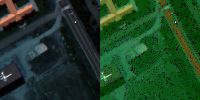
\includegraphics[width=0.75\textwidth]{segm_res.png}
\caption{Пример маски сегментации в результате работы программы}
\end{figure}

\begin{listing}[H]
    \caption{Пример выходного \texttt{json} файла}
    \label{lst:res_json_example}
    \begin{minted}[frame=single, breaklines, fontsize = \footnotesize, linenos]{python}
{
    "metric_value": 0.01668372569089048,
    "best_band": 41
}
    \end{minted}
\end{listing}

\anonsection{ЗАКЛЮЧЕНИЕ} %\anonsection{Заключение}

В ходе выполнения практической работы была разработана программа анализа гиперспектральных изображений с помощью осцилляторных нейронных сетей. Также была 
успешно реализована модульная система модели и одна из возможных стратегий выбора спектральных каналов.

\renewcommand\refname{СПИСОК ИСПОЛЬЗОВАННЫХ ИСТОЧНИКОВ}
\renewcommand{\mkgostheading}[1]{#1}
\renewcommand*{\newblockpunct}{\addperiod\addnbspace\textendash\space\bibsentence}
\renewcommand*{\bibrangedash}{\text{\textendash}}

% Список литературы
\clearpage
% \bibliographystyle{ugost2008s} %utf8gost71u.bst} %utf8gost705u} %gost2008s}
{\catcode`"\active\def"{\relax}
\addcontentsline{toc}{section}{\protect\numberline{}\refname}%
% \bibliography{biblio} %здесь ничего не меняем, кроме, возможно, имени bib-файла
\printbibliography
}

\end{document}